\documentclass[12pt]{article}
\usepackage[margin=1in]{geometry}
\usepackage[pdftex]{graphicx}
\usepackage{amsmath,amssymb,amsthm}
\usepackage{float}
\usepackage{custom}
\usepackage{pgfplots}
\usepackage{tikz}
\usepackage{tasks}
% \usepackage{times}
\usepackage{lmodern}

% color boxes
\usepackage[many]{tcolorbox}
\tcbuselibrary{theorems}
\newtcbtheorem{pssolution}{Solution}{colback=orange!10,colframe=orange!40!black,fonttitle=\bfseries,breakable,enhanced}{sn}
\tcbset{noparskip/.style={before={\par\pagebreak[0]\medskip\parindent=0pt},
after={\par\medskip}}}

% code for totaling up points 
\usepackage{totcount}
\newtotcounter{tpts}
\newtotcounter{cpts}
\newtotcounter{endpts}
\newcommand{\clearpts}{\addtocounter{tpts}{\value{cpts}} \setcounter{cpts}{0}}
\newcommand{\pts}[1]{\clearpts \setcounter{cpts}{#1}}
\newcommand{\totpts}{\setcounter{endpts}{\totvalue{tpts} + \totvalue{cpts}}\arabic{endpts}}

% formatting for problems and solutions
\definecolor{ptred}{rgb}{0.7,0.1,0.1}
\newcommand{\ptfmt}[1]{\textbf{\color{ptred}#1\color{black}}}
\definecolor{advblue}{rgb}{0.1,0.1,0.7}
\newcommand{\advanced}{\!\textbf{\color{advblue}[A]\color{black}}\ }

\newtheorem*{solution}{Solution}
\newtheorem*{answer}{Answer}

\makeatletter
\newtheoremstyle{mystyle}
{\topsep}               % space above
{\topsep}               % space below
{}                      % bodyfont
{}                      % indent
{\bfseries}             % headfont
{}                      % punctuation
{0.6em}                 % space after head
{\llap{[\ptfmt{\arabic{cpts}}]\hspace{.6em}}\thmname{#1}\thmnumber{ #2}\thmnote{\normalfont{ (#3)}}{\bfseries .}}  %theoremheadspec
\theoremstyle{mystyle}
\newtheorem{pproblem}{Problem}
\makeatother

% ------------- MOCK TITLE ------------- %
\newcommand\mocktitle{Momentum and Energy}
% -------------------------------------- %


% headers and footers
\usepackage{fancyhdr}
\pagestyle{fancy}
\lhead{\href{https://activities.tjhsst.edu/physics/index.html}{TJHSST Physics Team}}
\rhead{\thepage}
\cfoot{\href{https://activities.tjhsst.edu/physics/index.html}{TJHSST Physics Team}}
\renewcommand{\headrulewidth}{0.4pt}
\setlength{\headheight}{15pt}

\newcommand{\psettitle}[1]{
    \begin{center}
    \huge \textbf{#1}
    \end{center}
}

\linespread{1.03} % give a little extra room
\setlength{\parindent}{0.2in} % reduce paragraph indent a bit

% uncomment to hide solutions
% \usepackage{environ}
% \NewEnviron{hide}{}
% \let\solution\hide
% \let\endsolution\endhide
% \let\answer\hide
% \let\endanswer\endhide

% tikz setup
\usetikzlibrary{calc, decorations.pathreplacing, decorations.pathmorphing, angles, quotes, positioning}
\tikzstyle{arrow} = [thick,->,>=stealth]

\pgfplotsset{compat=1.18}

\begin{document}

\begin{center}
    \Large \textbf{\mocktitle\ Mock Exam} \vspace{4mm}
    
    \Large 10 MCQ 2 FRQ - 60 MINUTES \vspace{4mm}
    
    \Large \textbf{INSTRUCTIONS} \linebreak[2]
    
    \normalsize \textbf{DO NOT OPEN THIS TEST UNTIL YOU ARE TOLD TO BEGIN}
\end{center}

\begin{itemize}
    \item Use $g = 9.8$ N/kg throughout this contest.
    \item Test under standard conditions, meaning that you must complete the test in 60 minutes in one sitting.
    \item This test contains 10 Multiple Choice Questions, and 2 Free Response Questions.
    \item Correct answers will be awarded the points shown; Leaving an answer blank will be awarded zero points. The amount of partial credit is up to your discretion as the grader. Our recommendation is to be
    more strict than necessary.
    \item A hand-held calculator may be used. Its memory must be cleared of data and programs. You may use only the basic functions found on a graphing calculator. Calculators may not be shared. Cell phones may not be used during the exam. You may not use any tables, books, or collections of formulas.
    \item The number in \ptfmt{red} next to each question represents the amount of points the question is worth. There is a total of 40 points on this exam.
    \item While some problems may be solvable using Kinematics techniques, \textbf{it is generally advised to use theorems and equations pertaining to Momentum and Energy} to solve all problems. This is the sole focus of this unit and the AP Physics Teachers will likely omit credit unless this is done.
    \item If you have any questions, or clarifications, please contact us at \href{mailto:tjhsstphysicsteam@gmail.com}{tjhsstphysicsteam@gmail.com}.
\end{itemize}
\vspace{7mm}

The creators of this exam are (in alphabetical order):
\vspace{1mm}
% Please add your name in alphabetical order
\begin{center}
    \textit{Aarush Deshpande, Ryan Singh, Eric Xie}
\end{center}

Good luck, and have fun! Turn the page to start the mock.

\newpage

\subsection*{10 MCQs}


\pts{2}
\begin{pproblem}
    Two astronauts, Alice and Bob, are initially next to each other and both at rest in space. They suddenly push each other apart and, after one second, Alice is 12 m away from her starting point and Bob is 10 m away. Find the ratio of Alice's kinetic energy to Bob's kinetic energy ($K_A$/$K_B$).
    \begin{enumerate}[label=\Alph*)]
        \item $\dfrac{25}{36}$
        \item $\dfrac{5}{6}$
        \item $1$
        \item $\dfrac{6}{5}$
        \item $\dfrac{36}{25}$
    \end{enumerate}
\end{pproblem}
\begin{solution}
    Since we are given the distances after 1 second of each astronaut after one second, by allowing Alice to move in the positive $x$ direction, we have $v_A = 12$ m/s and  $v_B = 10$ m/s. From $KE = \dfrac{1}{2}mv^2$ and $p = mv$, we can find the relation of kinetic energy and momentum to be $KE = \dfrac{p^2}{2m}$. Since there are no external forces, we may observe by the conservation of momentum that the momenta of the two astronauts have equal magnitude and point in opposite directions. Therefore, $$\dfrac{K_A}{K_B} = \dfrac{p^2/2m_A}{p^2/2m_B} = \dfrac{m_B}{m_A}$$
    By conservation of momentum, find $12m_A = 10m_B$ so $\dfrac{m_B}{m_A} = \dfrac{6}{5}$. Since the ratio of the kinetic energies is $m_B/m_A$ as shown, our answer is \fbox{D: 6/5}
    
    Note: since the problem only asked for the ratio of Alice's and Bob's kinetic energies, we did not actually need to know their masses or velocities after applying conservation of momentum; we only needed the ratio of the masses which could be found using center of mass. 
\end{solution}

\pts{2}
% F=ma 2020 Q22
\begin{pproblem}
    A collision occurs between two masses. In each inertial reference frame, one can compute the change in total momentum $\Delta \v P$ and the change in total kinetic energy $\Delta K$ due to the collision. Which of the following is true?

    \begin{enumerate}[label=(\Alph*)]
        \item $\Delta \v P$ and $\Delta K$ do not depend on the frame.
        \item $\Delta \v P$ and $\Delta K$ do not depend on the frame
        for perfectly elastic collisions, but
        $\Delta \v P$ may depend on the frame for inelastic collisions.
        \item $\Delta \v P$ and $\Delta K$ do not depend on the frame
        for perfectly elastic collisions, but
        $\Delta K$ may depend on the frame for inelastic collisions.
        \item $\Delta \v P$ and $\Delta K$ do not depend on the frame
        for perfectly elastic collisions, but
        both may depend on the frame for inelastic collisions.
        \item $\Delta \v P$ and $\Delta K$ do not depend on the frame for perfectly elastic collisions, but both may depend on the frame for inelastic collisions
    \end{enumerate}
\end{pproblem}
\begin{solution}
    In a collision, momentum is always conserved so $\Delta\v P=0$ always.
    In any collision, any energy lost in the collision is released as heat, which is frame independent, so the answer is $\fbox{A}$.

    You can also show that $\Delta K$ is independent algebraically. Let \[
        \Delta K=\Delta K_m+\Delta K_M=\dfrac12mv_f^2-\dfrac12mv_0^2+\dfrac12Mu_f^2-\dfrac12Mu_0^2
    \]
    Now lets shift to a frame moving along the positive x-axis at a speed $q$.
    Our new $\Delta K$ then becomes \[
        \Delta K^\prime=\dfrac12m(v_f-q)^2-\dfrac12m(v_0-q)^2+\dfrac12M(u_f-q)^2-\dfrac12M(u_0-q)^2
    \]
    In combination with $mv_0+Mu_0=mv_f+Mu_f$, you should be able to verify that
    $\Delta K=\Delta K^\prime$
\end{solution}

\pts{2}
\begin{pproblem}
    A ball is dropped from a height $h$ and bounces on the ground. The
    velocity of the ball after it bounces off the ground for the $n$th time
    is $v_n=\alpha v_{n-1}$, where $0<\alpha\le1$. Take the system of the 
    ball and the earth: which of the following graphs
    could show the mechanical energy of the system as a function of time?

    \begin{tasks}[label=(\Alph*),label-width=20pt](2)
        \task
        \begin{tikzpicture}
          \draw[->] (0, 0) -- (2.2, 0) node[right] {$t$};
          \draw[->] (0, 0) -- (0, 2.2) node[above] {$E$};
          \draw[domain=0:2, smooth, variable=\x, blue] plot ({\x}, {2-\x});
        \end{tikzpicture}
        
        \task
        \begin{tikzpicture}
          \draw[->] (0, 0) -- (2.2, 0) node[right] {$t$};
          \draw[->] (0, 0) -- (0, 2.2) node[above] {$E$};
          \draw[domain=0:2, smooth, variable=\x, blue] plot
            ({\x}, {2^(-2*\x+1)});
        \end{tikzpicture}

        % This is the correct answer, but it could look way better
        % maybe don't show the x-axis intersection?
        \task
        \begin{tikzpicture}
          \draw[->] (0, 0) -- (2.2, 0) node[right] {$t$};
          \draw[->] (0, 0) -- (0, 2.2) node[above] {$E$};
          \draw[blue] (0, 2) -- (0.5, 2) -- (0.5, 1.5) -- (1, 1.5) -- (1, 1) -- (1.5, 1) -- (1.5, 0.5) -- (2, .5);
        \end{tikzpicture}

        \task
        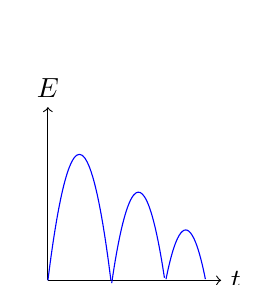
\begin{tikzpicture}
          \draw[->] (0, 0) -- (2.2, 0) node[right] {$t$};
          \draw[->] (0, 0) -- (0, 2.2) node[above] {$E$};
          \draw[domain=0:0.8, smooth, variable=\x, blue] plot
            ({\x}, {1.6-10*(\x-0.4)^2});
          \draw[domain=0.81:1.48, smooth, variable=\x, blue] plot
            ({\x}, {1.12-10*(\x-1.15)^2});
          \draw[domain=1.5:2, smooth, variable=\x, blue] plot
            ({\x}, {0.64-10*(\x-1.75)^2});
        \end{tikzpicture}

        \task
        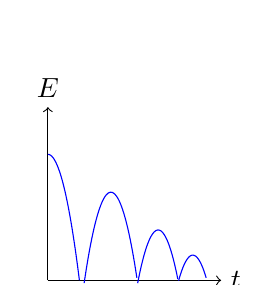
\begin{tikzpicture}
          \draw[->] (0, 0) -- (2.2, 0) node[right] {$t$};
          \draw[->] (0, 0) -- (0, 2.2) node[above] {$E$};
          \draw[domain=0:0.4, smooth, variable=\x, blue] plot
            ({\x}, {1.6-10*\x^2});
          \draw[domain=0.46:1.13, smooth, variable=\x, blue] plot
            ({\x}, {1.12-10*(\x-0.8)^2});
          \draw[domain=1.14:1.65, smooth, variable=\x, blue] plot
            ({\x}, {0.64-10*(\x-1.4)^2});
          \draw[domain=1.66:2.01, smooth, variable=\x, blue] plot
            ({\x}, {0.32-10*(\x-1.84)^2});
        \end{tikzpicture}
    \end{tasks}
\end{pproblem}
\begin{solution}
    Every time the ball hits the ground, a partially inelastic collision occurs. The ball loses energy (in the form of heat), so the overall mechanical energy of the ball should be going down. Additionally, it only loses energy when it collides with the ground (the up and down motion of the ball is just a conversion between kinetic and potential energy as the only force acting upon the ball is gravity, which is conservative), so the energy should decrease in discrete steps, or option \fbox{C}.
\end{solution}

\pts{2}
\begin{pproblem}
    A small block of mass 1 kg slides on an icy surface with a velocity of 10 m/s to the east. It is attached by a rope of length 4 meters (there is initially some slack in the rope) to a small pole as shown. At time A, the center of the block is 2 meters directly south of the pole. At time B, the rope suddenly becomes taut and does not stretch. Find the magnitude (to the nearest hundredth) and direction of the impulse the block experiences.
    \begin{figure}[H]
        \centering
        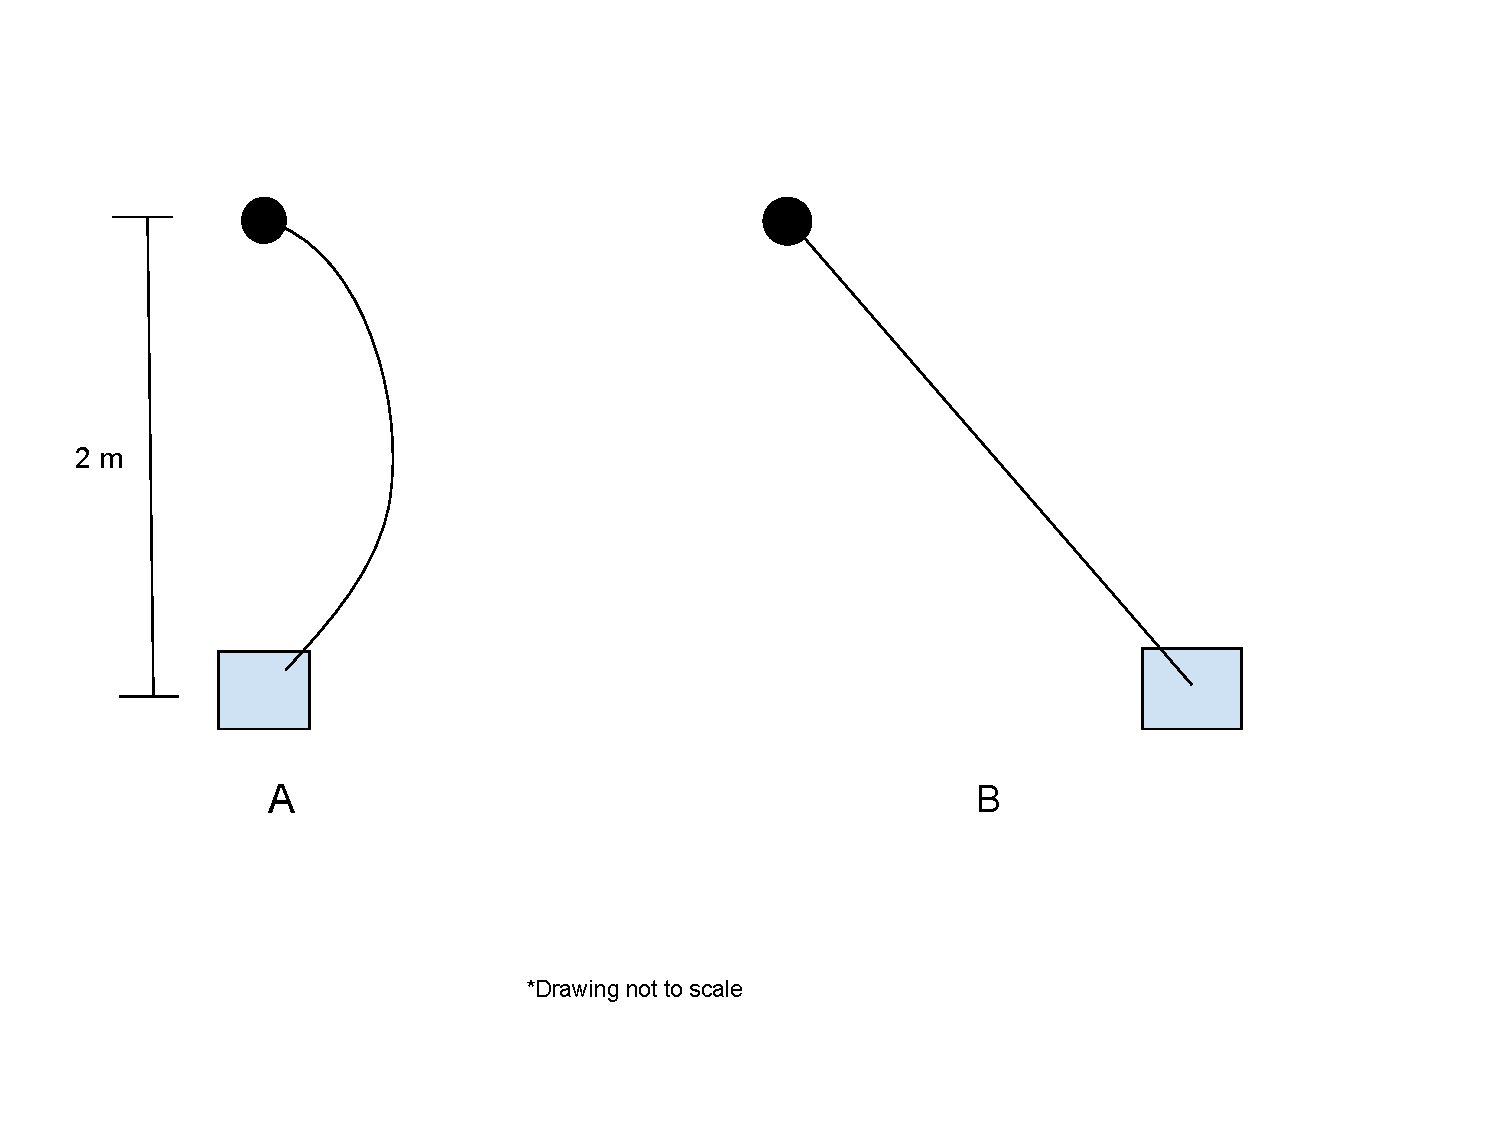
\includegraphics[scale=0.6]{images/block_and_pole.pdf}
    \end{figure}
    \begin{enumerate}[label=\Alph*)]
        \item 5 Newton-seconds towards the pole
        \item 5 Newton-seconds west
        \item 5 Newton-seconds north-east (perpendicular to the line from block to pole)
        \item 8.66 Newton-seconds towards the pole
        \item 8.66 Newton-seconds west
        \item 10 Newton-seconds towards the pole
        \item 10 Newton-seconds west
    \end{enumerate}
\end{pproblem}
\begin{solution}
    The only force of note acting on the block is the tension force in the rope after it goes taut, which points along the rope and towards the pole. Since impulse is given by $\vec{J} = \int_{t_i}^{t_f} \vec{F} dt$, the impulse points in the same direction as the force, so it must also point towards the pole. We can therefore rule out answer choices B, C, E, and G. 
    
    To find the magnitude of the impulse, we first break the block's velocity right before time B into radial and tangential components relative to the pole. Since the block is 2 meters south of the pole, and the rope is 4 meters long, the angle between the rope and the horizontal (east-west) axis is 30 degrees. Therefore, the component of the velocity pointing parallel to the rope is $v\cos 30 = 10\cos30 = 8.66$ m/s. After the rope goes taught, the radial velocity becomes 0, since the rope cannot stretch. Therefore, the magnitude of the change in momentum is $|1*(0-8.66)| = 8.66$ Newton-seconds. The velocity in the tangential direction does not change, since the tension in the rope points only in the radial direction and cannot exert a force in the tangential direction. Therefore, the answer is \fbox{D}
\end{solution}


% source: some F=ma question somewhere
\pts{2}
\begin{pproblem}
    A balloon is filled with helium at the bottom of a room and floats to the ceiling. In other words, the gravitational potential energy of the balloon increased. Since mechanical energy is conserved, something else must have decreased during this process. Which of the following is the main contribution to this decrease?
    \begin{enumerate}[label=\Alph*)]
        \item The kinetic energy of the balloon decreased.
        \item The elastic potential energy of the balloon decreased.
        \item The thermal energy of the air in the balloon decreased.
        \item The thermal energy of the air in the room decreased.
        \item The gravitational potential energy of the air in the room decreased.
    \end{enumerate}
\end{pproblem}
\begin{solution}
    The reason the balloon is able to float is that more dense air is able to sink and fill up the volume of where the balloon was. Therefore, the answer is \fbox{E}. Another way to think about this problem is to observe that when the balloon floats to the ceiling, it displaces some of the air that was already there and this air then displaces the balloons initial position at the bottom of the room. Therefore, the height of this air decreases, decreasing its gravitational potential energy.
\end{solution}

\pts{2}
\begin{pproblem}
    A train of mass $M$ is driving horizaontally at a velocity $v$. Snow falls vertically on the train at a rate of $\rho$ kg/s. What is the power required to keep the train traveling at a constant speed $v$?
    \begin{enumerate}[label=\Alph*)]
        \item 0
        \item $Mgv$
        \item $\dfrac{1}{2}Mv^2$
        \item $\dfrac{1}{2}\rho v^2$
        \item $\rho v^2$
    \end{enumerate}
\end{pproblem}
\begin{solution}
    Take a period of time $t$ in which snow of mass $m = \rho t$ falls onto the train. The impulse exerted by the train to bring the snow from a horizontal speed of $0$ to $v$ is then $J=\rho t v$. The force is then $F = J/t = \rho v$,
    and using $P = F\cdot v$ we have the answer as \fbox{E: $\rho v^2$}
\end{solution}

\pts{2}
\begin{pproblem}
    A small bead is placed on the top of a frictionless glass sphere of
    diameter $D$. The bead is given a slight push and starts sliding
    down along the sphere. Find the speed $v$ of the bead at the point
    at which the bead leaves the sphere.

    \begin{figure}[H]
        \centering
        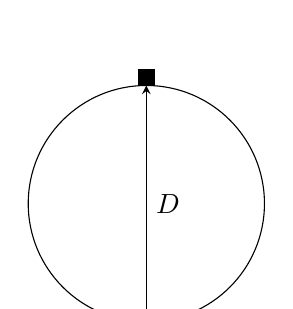
\begin{tikzpicture}
            \draw (0,0) circle (1.5);
            \filldraw (-0.1,1.5) rectangle (0.1,1.7);
            \draw[stealth-stealth] (0, -1.5) -- (0, 1.5)
                node[midway, right] {$D$};
        \end{tikzpicture}
    \end{figure}

    \begin{tasks}[label=(\Alph*),label-width=20px](3)
        \task $v=\sqrt{gD}$
        \task $v=\sqrt{4gD/5}$
        \task $v=\sqrt{2gD/3}$
        \task $v=\sqrt{gD/2}$
        \task $v=\sqrt{gD/3}$
    \end{tasks}
\end{pproblem}
\begin{solution}
    Let the bead leave the sphere at an angle $\theta$ to the vertical.
    By conservation of energy, we have \[
        mgr=mgr\cos\theta+\dfrac{1}{2}mv^2
    \]
    where $r=D/2$ is the radius of the sphere. In order for the block to
    move along the sphere, it has to have a net centripetal force $mv^2/r$.
    From $F=ma$ we have \[
        mg\cos\theta-N=mv^2/r
    \]
    At the critical point where the bead leaves the sphere, we have $N=0$
    and $mg\cos\theta=mv^2/r$.
    Solving the system of equations gives \[
        v=\sqrt{\dfrac{2}{3}gr}=\sqrt{\dfrac{gD}3}
    \]
    or answer choice \fbox{E}.
\end{solution}

\pts{2}
\begin{pproblem}
    A block of mass 5 kg with a horizontal velocity of 8 m/s and no vertical velocity explodes into two pieces that initially fly apart at right angles to each other. One piece has a mass of 1.5 kg and a velocity of 11 m/s. Which of the options is closest to the change in kinetic energy of the system?
    \begin{enumerate}[label=(\Alph*)]
        \item $-85$ J
        \item $0$ J
        \item $60$ J
        \item $120$ J
        \item $310$ J
    \end{enumerate}
\end{pproblem}
\begin{solution}
    Letting the initial momentum of the block be $\vec{p_0}$, and letting the magnitudes of the momenta of the fragments be $\vec{p_1}$ and $\vec{p_2}$, we claim that $p_0^2 = p_1^2 + p_2^2$. 

    One way to show this is by breaking the momenta into components in the horizontal and vertical directions. Assume the first fragment flies away at an angle of $\theta$ above the horizontal, so $\vec{p_1}$ points $\theta$ degrees above the horizontal, and the x and y components of the momentum are,
    \begin{align*}
        p_{1x} &= p_1 \cos \theta\\
        p_{1y} &= p_1 \sin \theta
    \end{align*}
    Since the two fragments travel at right angles to each other, $\vec{p_2}$ points $90 - \theta$ degrees below the horizontal. Using the trig identity $\sin (90-\theta) = \cos \theta$ and $\cos (90-\theta) = \sin\theta$, the components of $\vec{p_2}$ are
    \begin{align*}
        p_{2x} &= p_2 \sin \theta\\
        p_{2y} &= -p_2 \cos \theta
    \end{align*}
    The initial momentum in the y direction is 0, so by conservation of momentum, $p_1 \sin \theta-p_2 \cos \theta = 0$ so $$p_1 \sin \theta = p_2 \cos \theta$$
    The initial momentum in the x direction is $p_0$ so $$p_1 \cos \theta + p_2 \sin \theta = p_0$$
    Solving the system of equations, 
    \begin{align*}
        p_0^2&=p_1^2\cos^2\theta + p_1p_2\sin\theta\cos\theta
            + p_1p_2\sin\theta\cos\theta + p_2^2\sin^2\theta\\
        &=p_1^2\cos^2\theta + p_1^2\sin^2\theta + p_2^2\cos^2\theta
            + p_2^2\sin^2\theta\\
        &=p_1^2 + p_2^2
    \end{align*}

    Alternatively, this result can also be shown by using $\vec{p_0} = \vec{p_1} + \vec{p_2}$. Since $\vec{p_1}$ and $\vec{p_2}$ are at right angles, $p_0$, $p_1$, and $p_2$ are the side lengths of a right triangle, so applying the Pythagorean theorem leads to the same result. 

    Since the masses and velocities of the initial block and the first fragment are known, we can calculate (eliding units) $p_0 = 40$ and $p_1 = 16.5$. Using the above result gives $p_2 = 36.4$.
    
    From $K = \dfrac{1}{2}mv^2$ and $p = mv$, we find the relation $K = \dfrac{p^2}{2m}$. From this, we find the initial kinetic energy is $K_0 = \dfrac{40^2}{2\cdot5} = 160$ J and the final kinetic energy is $K_f = \dfrac{16.5^2}{2\cdot1.5} + \dfrac{36.4^2}{2\cdot3.5} = 280$ J. The change in kinetic energy is then $\Delta K = 120 \text{ J}$, or \fbox{D}
\end{solution}

% 2016 F=ma 13
\pts{2}
\begin{pproblem}
    An object of mass $m_1$ initially moving at speed $v_0$ collides with
    an originally stationary object of mass $m_2 = \alpha m_1$, where
    $\alpha < 1$. The collision could be completely elastic, completely
    inelastic, or partially inelastic. After the collision, the two
    objects move at speeds $v_1$ and $v_2$. Assume that the
    collision is one dimensional, and that object one cannot pass
    through object two. After the collision, the speed ratio
    $r_2 = v_2/v_0$ of object 2 is bounded by:
    \begin{enumerate}[label=\Alph*)]
        \item $1/(1+\alpha)\le r_2 \le 2/(1+\alpha)$
        \item $(1-\alpha)/(1+\alpha)\le r_2\le 1$
        \item $(1-\alpha)/(1+\alpha)\le r_2\le 1/(1+\alpha)$
        \item $\alpha/(1+\alpha)\le r_2\le 1$
        \item $0\le r_2 \le 2\alpha/(1+\alpha)$
    \end{enumerate}
\end{pproblem}
\begin{solution}
    The solution will be bounded by the speed ratio for a perfectly elastic
    and perfectly inelastic collision. A partially inelastic collision
    will fall somewhere in the range between the two. Let's start with a
    perfectly inelastic collision, which will be our lower bound.

    In a perfectly inelastic collision, the masses will move at the speed
    of their center of mass after the collision. This gives us
    \begin{align*}
        v_2&=\dfrac{m_1v_0}{m_1+\alpha m_1}=\dfrac{v_0}{1+\alpha}\\
        \implies r_2&=\dfrac{v_2}{v_0}=\dfrac{1}{1+\alpha}
    \end{align*}

    In a perfectly elastic collision, in the frame of the center of mass,
    all that happens is the momentum of mass $m_2$ flips direction. Using this, we can find $v_2$ for an elastic collision.
    
    Let's start by finding the velocity of $m_2$ in the frame of the center of mass: \[
        v_\mathrm{2,cm}=0-\dfrac{m_1v_0}{m_1+\alpha m_1}=-\dfrac{v_0}{1+\alpha}
    \]
    After the collision, its velocity will flip direction: \[
        v_\mathrm{2f,cm}=-\left(-\dfrac{v_0}{1+\alpha}\right)=\dfrac{v_0}{1+\alpha}
    \]
    Finally, we can add the velocity of the center of mass to convert back
    to the lab frame
    \[
        v_\mathrm{2,f}=\dfrac{v_0}{1+\alpha}
            +\dfrac{v_0}{1+\alpha}=\dfrac{2v_0}{1+\alpha}
    \]
    And so $r_2=v_2/v_0=2/(1+\alpha)$, giving us our final inequality of \[
        \dfrac{1}{1+\alpha}\le r_2 \le \dfrac{2}{1+\alpha}
    \] or \fbox{A}.
\end{solution}

% we can make this harder if neccessary
% I couldn't think of anything better, so for now it's just a calculator
% bash
% ---------------------------------------------------------------------
% yeah I really hate this
% ---------------------------------------------------------------------
\begin{pproblem}
    A block of mass $1$ kg initially has a velocity $4.9$ m/s down an inclined plane of angle $50^\circ$. The block is attached to a spring of spring constant $9\mathrm{kg/s^2}$, which is initially at it's relaxed length. The coefficient of kinetic and static friction between the block and the plane are $\mu$. Given that the lowest position on the plane the block will reach is $5$m along the plane, which of the following is the closest to
    the value of $\mu$?

    % yes I got lazy and this is really bad tikz code/diagram
    \begin{figure}[H]
        \centering
        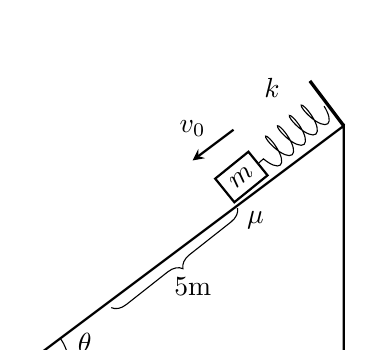
\begin{tikzpicture}
            \coordinate (a) at (0, 0);
            \coordinate (b) at (4, 0);
            \coordinate (c) at (4, 3);
            \draw[thick] (a) -- (b) -- (c) -- cycle;
            \draw[very thick] (4, 3) -- (3.57, 3.57);
            \node (m) at (2.7,2.35) [draw,thick,minimum width=.2cm,minimum height=.2cm,rotate=39] {$m$};
            \draw[arrow] (2.6,2.95) -- (2.08,2.56) node[above=5px] {$v_0$};
            \draw[decoration={aspect=0.3, segment length=2mm, amplitude=2mm,coil},decorate] (3.75,3.25) -- (m.east);
            \node at (3.09,3.48) {$k$};
            \node at (2.88,1.8) {$\mu$};

            \pic[draw, -, "$\theta$", angle eccentricity=1.5] {angle = b--a--c};
            \draw [decorate,decoration={brace,amplitude=5pt,raise=.5ex}]
                (m.215) -- (1,0.75)
                node[midway,yshift=-1.2em,xshift=.8em]{$5$m};
        \end{tikzpicture}
    \end{figure}

    \begin{tasks}[label=(\Alph*),label-width=20px](5)
        \task 1
        \task 2
        \task 3
        \task 4
        \task 5
    \end{tasks}
\end{pproblem}
% let's be honest, I probably messed up putting stuff into the calculator
% someone please double check
\begin{solution}
    We can use the work energy theorem here, letting $x$ be the distance traveled along the plane.
    
    First observe that the final kinetic energy must be 0, as the block comes to rest. The change in potential energy comes from the drop in the gravitational potential energy of the box and the addition of the elastic potential energy from the spring. The potential energy of a spring is $kx^2/2$, and since the spring is initially at relaxed length this is the total increase from the spring. Since the height of the box changes, we can calculate the drop in gravitational potential energy to be $mg\Delta h$. Since the box traveled a distance of $x$ along the box, $\Delta h = x\sin\theta$, so gravitational potential energy decreases by $mgx\sin\theta$. We can calculate the total work done by friction as $F_{friction} \cdot x = \mu N \cdot x = \mu mg\cos\theta \cdot x$. Thus, we have:
    \begin{align*}
        W_\mathrm{friction}&=\Delta K+\Delta U
            = \left(0 -\dfrac{1}{2}mv_0^2\right) + \left(\dfrac{1}{2}kx^2 - mgx\sin\theta\right)\\
        \implies \mu mgx\cos\theta&=
            -\dfrac{1}{2}mv_0^2-mgx\sin\theta+\dfrac{1}{2}kx^2
    \end{align*}
    Solving for $\mu$ gives \[
        \mu=\dfrac{kx^2-mv_0^2-2mgx\sin\theta}{2mgx\cos\theta}
    \]
    Plugging in values gives us $\mu\approx 2$, or \fbox{B}.
\end{solution}


\subsection*{2 Free Responses}
\setcounter{pproblem}{0}


% Problem is taken from Morin, Problems and Solutions in Introductory Mechanics
% but sol is handwritten by Aarush
\pts{10}
\begin{pproblem}
    A stream of $N$ clay balls of mass $m$ move with a speed $v$ in a line
    across a frictionless table. The spacing between them in $\ell$. An
    additional ball of mass $m$ sits in front of them. The front ball collides
    with the stationary ball and forms a blob of mass $2m$. Then the second
    ball collides with the blob and forms a blob of mass $3m$, and so on.
    How much time elapses between the instant shown below (when all balls are
    separated by a distance $\ell$) and the last collision?

    Solve this by working in:
    \begin{enumerate}[label=\Alph*)]
        \item The lab frame
        \item The frame in which the $N$ balls are initially at rest.
        \item If instead of having equally distributed mass, imagine each ball has more mass than the previous ball. Will the collisions then take more, less, or the same amount of time? In this case, the stationary ball has mass $m$, and the first ball to collide has mass $am$ where $a > 1$, and each succeeding ball has a greater mass than the previous ball. Give a formulaic explanation for full credit.
    \end{enumerate}

    \begin{figure}[H]
        \centering
        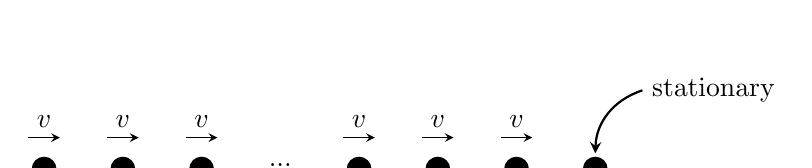
\begin{tikzpicture}
            \foreach \i in {1,...,3} {
                \filldraw (\i,0) circle (0.15);
                \draw[-stealth] (\i-0.2, 0.4) -- (\i+0.2, 0.4) node[above, midway] {$v$};
            }
            \node at (4,0.05) {$...$};
            \foreach \i in {1,...,3} {
                \filldraw (4+\i,0) circle (0.15);
                \draw[-stealth] (4+\i-0.2, 0.4) -- (4+\i+0.2, 0.4) node[above, midway] {$v$};
            }
            \filldraw (8,0) circle (0.15);
            \node (label) at (9.5, 1) {stationary};
            \draw[arrow] (label.west) to[bend right=35] (8,0.2);
        \end{tikzpicture}
    \end{figure}
\end{pproblem}
\begin{solution}
    \begin{enumerate}[label=\Alph*)]
        \item 
        Each collision to form a blob is an inelastic collision, which means
        that the resulting blob moves at the same velocity as the center of
        mass of the balls that form the blob. As such, the velocity of the blob
        after $n$ balls have formed into the blob is given by \[
            v_n=\dfrac{n-1}{n}v
        \]
        \begin{remark}
            You can also derive this via conservation of momentum. Suppose we
            have $n$ balls, of which one is stationary. At the end of the collision,
            they all move at the same velocity $v_n$. Thus, we have the equation \[
                (n-1)v=nv_n\implies v_n=\dfrac{n-1}{n}v
            \]
            in agreement with above.
        \end{remark}

        The relative velocity between the $n$th ball and the blob is then \[
            v_\text{rel,n}=v-\dfrac{n-1}{n}v=\dfrac{v}{n}
        \]
        Given $v_n$, the time taken for the $n$th ball to collide is \[
            t_n=\dfrac{\ell}{v_\text{rel,n}}=\dfrac{n\ell}{v}
        \]
        The total time is just a sum of $t_n$ from $n=1$ to $n=N$:
        \begin{align*}
            T&=\sum_{n=1}^N\dfrac{n\ell}{v}\\
            &=\dfrac{\ell}{v}\sum_{n=1}^Nn\\
            &=\boxed{\dfrac{\ell}{v}\left(\dfrac{N(N+1)}{2}\right)}
        \end{align*}
        The last equality comes from the sum of an arithmetic sequence.

        \item 
        In this frame, the last ball is moving left with a velocity $v$,
        while all other balls are stationary. By the definition of an 
        inelastic collision (or conservation of momentum if you prefer), the 
        velocity after $n-1$ collisions (or of a blob of $n$ balls) is just \[
            (nm)v_n=mv\implies v_n=\dfrac{v}{n}
        \]
        Thus we have (by the logic in the previous section): 
        \begin{align*}
            t_n&=\dfrac{\ell}{v_n}=\dfrac{n\ell}{v}\\
            T&=\sum_{n=1}^N\dfrac{n\ell}{v}\\
            &=\boxed{\dfrac{\ell}{v}\left(\dfrac{N(N+1)}{2}\right)}
        \end{align*}
        In agreement with our previous result.

        \item Let the mass of the stationary ball be $m$ and the mass of the first ball to collide be $am$ where $a > 1$. After collision with the stationary ball, by conservation of momentum, we have 
        \[amv = (1+a)mv_f\]
        \[v_f = \frac{av}{a+1}\]
        The relative velocity of the second ball to collide to the new blob is  \[
            v_\text{rel,2}=v-\dfrac{va}{a+1}=\dfrac{v}{a+1}
        \]
        Then we solve for the time needed for the collision: \[
            t_2=\dfrac{\ell}{v_\text{rel,2}}=\dfrac{\ell}{v}(a+1)
        \]
        Given $a > 1$, we know that the $t_2$ in this case is greater than what is used to be for the 2nd ball, which was $\frac{n\ell}{v} = \frac{2\ell}{v}$. We can extrapolate this for all $N$ balls as the masses increase with each one. Therefore, the collisions will take \fbox{more time}.
        
    \end{enumerate}
\end{solution}

\pts{10}
\begin{pproblem}
    A hose shoots a stream of water vertically upward. The water leaves the
    hose at a velocity $v_0$ and at a mass rate $R$ (kg/s).
    \begin{enumerate}[label=\Alph*)]
        \item A horizontal board with mass $m$ is placed a very small distance
        above the hose and then released. What should $m$ be so that the
        board hovers at this height? Assume that when the water crashes into
        the board, it bounces off essentially sideways. Solve in terms of given variables and fundamental constants.

        \item If you break the board in half, so that its mass is now $m/2$,
        how high above the hose will it be located such that it will
        hover in place? Solve in terms of given variables and fundamental constants.

        \item In part (A), what should $m$ be if the stream of water is
        replaced by a stream of marbles that bounce off the board elastically
        (that is, they bounce off downward with the same speed $v_0$)? Solve in terms of given variables and fundamental constants.

        (Even though the marbles are discrete objects, assume that they have
        an essentially continuous mass rate equal to $R$. Also, assume that the
        downward-moving marbles that have bounced off the board somehow
        magically pass through the upward-moving ones without colliding.)
    \end{enumerate}
\end{pproblem}
\begin{solution}
    \begin{enumerate}[label=\Alph*)]
        \item Take a small packet of water, $\delta m=R\delta t$
        \footnote{$\delta m$ is used to indicate a \textit{small} amount of mass,
        and $\delta t$ is used to indicate a \textit{small} change in time.}.
        The momentum of this packet of water is given by
        $v_0\delta m=v_0R\delta t$. The impulse provided upon hitting the
        board is then $J=0-v_0R\delta t=-v_0R\delta t$, since the water has 0 vertical velocity after hitting the board.
        Since the board is suspended in place, this must be equal to the impulse due to gravity, which is
        $-mg\delta t$. Therefore, we have \[
            -mg\delta t=-v_0R\delta t\implies \boxed{m=\dfrac{v_0R}{g}}
        \]

        \item 
        From part (A) we know that the velocity needed to support a board of
        mass $m/2$ is
        \begin{align*}
            \dfrac{m}{2}=\dfrac{vR}{g}
                \implies v=\dfrac{mg}{2R}=\dfrac{v_0}{2}
        \end{align*}
        Using conservation of energy, we can find the height:
        \begin{align*}
            \dfrac{1}{2}(R\delta t)v_0^2&=(R\delta t)gh+\dfrac{1}{2}(R\delta t)\left(\dfrac{v_0}{2}\right)^2\\
            \implies h&=\dfrac{3v_0^2}{8g}
        \end{align*}

        \item 
        If marbles bounce off the board elastically, then the only
        difference is that they give off a larger impulse to keep the
        board afloat. When it bounces off the board, all that happens is
        its velocity flips directions. 
        In such a case, we have the impulse as \[
            J= -v_0R\delta t-v_0R\delta t=-2v_0R\delta t
        \]
        Setting up our equation with the impulse due to gravity, we get
        the new result
        \begin{align*}
            -mg\delta t=-2v_0R\delta t\implies\boxed{m=\dfrac{2v_0R}{g}}
        \end{align*}
    \end{enumerate}
\end{solution}


\end{document}
